\documentclass{article}

\usepackage{arxiv}

\usepackage[utf8]{inputenc} % allow utf-8 input
\usepackage[T1]{fontenc}    % use 8-bit T1 fonts
\usepackage{lmodern}        % https://github.com/rstudio/rticles/issues/343
\usepackage{hyperref}       % hyperlinks
\usepackage{url}            % simple URL typesetting
\usepackage{booktabs}       % professional-quality tables
\usepackage{amsfonts}       % blackboard math symbols
\usepackage{nicefrac}       % compact symbols for 1/2, etc.
\usepackage{microtype}      % microtypography
\usepackage{graphicx}

\title{Predictive Approaches to Treatment Effect Heterogeneity}

\author{
    Tom Delany
    \thanks{Use footnote for providing further information about author
(webpage, alternative address)---\emph{not} for acknowledging funding
agencies. Optional.}
   \\
    Department of Mathematical and Statistical Sciences \\
    University of Galway \\
  Galway, Ireland \\
  \texttt{\href{mailto:d.tom2@universityofgalway.ie}{\nolinkurl{d.tom2@universityofgalway.ie}}} \\
   \And
    Misgana Ojamo
   \\
    Department of Mathematical and Statistical Sciences \\
    University of Galway \\
  Galway, Ireland \\
  \texttt{\href{mailto:M.Ojamo1@universityofgalway.ie}{\nolinkurl{M.Ojamo1@universityofgalway.ie}}} \\
  }


% tightlist command for lists without linebreak
\providecommand{\tightlist}{%
  \setlength{\itemsep}{0pt}\setlength{\parskip}{0pt}}


% Pandoc citation processing
%From Pandoc 3.1.8
% definitions for citeproc citations
\NewDocumentCommand\citeproctext{}{}
\NewDocumentCommand\citeproc{mm}{%
  \begingroup\def\citeproctext{#2}\cite{#1}\endgroup}
\makeatletter
 % allow citations to break across lines
 \let\@cite@ofmt\@firstofone
 % avoid brackets around text for \cite:
 \def\@biblabel#1{}
 \def\@cite#1#2{{#1\if@tempswa , #2\fi}}
\makeatother
\newlength{\cslhangindent}
\setlength{\cslhangindent}{1.5em}
\newlength{\csllabelwidth}
\setlength{\csllabelwidth}{3em}
\newenvironment{CSLReferences}[2] % #1 hanging-indent, #2 entry-spacing
 {\begin{list}{}{%
  \setlength{\itemindent}{0pt}
  \setlength{\leftmargin}{0pt}
  \setlength{\parsep}{0pt}
  % turn on hanging indent if param 1 is 1
  \ifodd #1
   \setlength{\leftmargin}{\cslhangindent}
   \setlength{\itemindent}{-1\cslhangindent}
  \fi
  % set entry spacing
  \setlength{\itemsep}{#2\baselineskip}}}
 {\end{list}}
\usepackage{calc}
\newcommand{\CSLBlock}[1]{#1\hfill\break}
\newcommand{\CSLLeftMargin}[1]{\parbox[t]{\csllabelwidth}{#1}}
\newcommand{\CSLRightInline}[1]{\parbox[t]{\linewidth - \csllabelwidth}{#1}\break}
\newcommand{\CSLIndent}[1]{\hspace{\cslhangindent}#1}

\providecommand{\pandocbounded}[1]{#1}
\usepackage[HTML]{xcolor}
\usepackage{booktabs}
\usepackage{caption}
\usepackage{longtable}
\usepackage{colortbl}
\usepackage{array}
\usepackage{anyfontsize}
\usepackage{multirow}
\begin{document}
\maketitle


\begin{abstract}
Enter the text of your abstract here.
\end{abstract}

\keywords{
    blah
   \and
    blee
   \and
    bloo
   \and
    these are optional and can be removed
  }

\section{Introduction}\label{introduction}

\subsection{Clinical Motivation}\label{clinical-motivation}

The majority of treatment decisions made by regulatory bodies, payers,
physicians and other stakeholders is based on data pertaining to average
treatment effects Willke et al. (2012). Randomised-controlled trials
remain the gold-standard for the determination of casual effects.
Reliance on average effects from small cohorts of selected participants
in clinical trial is not always representative of the effects in an
individual patient. This nonrandom variance in the magnitude and
direction of treatment effects between individuals is referred to as the
heterogeneity of treatment effect.

This is not a contemporary observation and is one that was identified
long before formal statistical approaches to model this heterogeneity
were deployed Albert, Gadbury, and Mascha (2005). Currently, subgroup
analyses are the most common method of exploring treatment-effect
heterogeneity in clinical trials. The approach involves dividing trial
participants into groups defined by a particular characteristic such as
Sex or Age. Subgroup analyses are simple to implement and easily
interpretable to key stakeholders, however, they can suffer from a
number of limitations. Well-established limitations include high rates
of false positives and negatives and their inability to inform
individual treatment decisions. These analyses generally consider one
factor at a time and therefore cannot account for the fact that patients
have multiple characteristics that jointly influence treatment response
Kent et al. (2020). Recently there has been increased interest in
multivariate models for treatment effect heterogeneity.

\subsection{Predictive Approaches to Treatment Effect
Heterogeneity}\label{predictive-approaches-to-treatment-effect-heterogeneity}

Predictive approaches to treatment effect heterogeneity (PATH) are
methods of increasing importance in precision medicine, designed to
determine the reason for different responses in patients to the same
treatment. To achieve this, risk- and effect-based models are
constructed, aiming to provide a patient's expected outcome at the
individual level with versus without treatment. These models incorporate
all relevant patient attributes simultaneously, allowing for a
comprehensive characterization of inter-individual differences in
treatment effect.

\subsection{Methods to employ PATH}\label{methods-to-employ-path}

There are two approaches to predictive HTE analysis: risk-based
modelling and effects-based modelling. Risk-based modelling involves
constructing a multivariable model that predicts individual baseline
risk, after which treatment effects are examined across strata of
predicted risk. Effects-based modelling, in contrast, involves the
direct estimation of individual treatment effects and is often performed
using regression models, though more recently nonparametric
machine-learning algorithms have been applied. At the time of the
release of the PATH statement in 2020, risk-based modelling was the more
substantiated of the two approaches, while effects-based models were
viewed as promising---particularly in larger datasets. In recent years,
there has been growing interest in reducing model overfitting in
effects-based models. Overfitting occurs when a model begins to describe
random error rather than true relationships between variables,
substantially reducing its generalizability. The following section will
discuss both risk-based and effects-based approaches in more detail,
outlining their use cases, limitations, and how future developments may
guide their clinical deployment.

\subsection{Risk-Based}\label{risk-based}

Risk-based approaches stratify patients according to their baseline risk
of the primary trial outcome. Stratification is typically performed
using an existing or an in-house multivariable prediction model, from
which estimates of relative and absolute treatment effects are computed
across prespecified risk strata. This approach is practical and
clinically important because a patient's baseline risk of experiencing a
bad outcome without treatment determines the absolute benefit they can
gain from therapy. Since absolute benefit, defined as the difference in
risk between receiving and not receiving treatment, is mathematically
tied to baseline risk, stratifying patients often reveals meaningful
variations in benefit. For example, a patient at very low risk may gain
little absolute benefit, and if the treatment carries even a small risk
of harm, the trade-off may be unfavourable.

\subsection{Effect-Models}\label{effect-models}

Effects-based models involve the construction of a regression model
directly on randomized controlled trial data, where individual treatment
effects are estimated using multivariate regression that includes
treatment, covariate, and interaction terms. Non-parametric machine
learning approaches have also been used to examine individual treatment
effects, including reward-based Q-learning techniques. This approach
develops models directly on trial data to predict treatment effects by
including terms for factors that might change the relative effectiveness
of the treatment. While promising, these models can be complex and are
vulnerable to statistical issues such as overfitting, where results
appear strong in the analysed data but do not predict accurately in new
patients.

\subsection{Clinical Relevance of
PATH}\label{clinical-relevance-of-path}

Enables precision medicine and personalized treatment.

\subsection{PATH Reporting}\label{path-reporting}

Standardized reporting guidance (PATH statement).

\subsection{Context of Datasets}\label{context-of-datasets}

\begin{table}[t]
\fontsize{8.0pt}{9.0pt}\selectfont
\begin{tabular*}{525pt}{@{\extracolsep{\fill}}>{\raggedright\arraybackslash}p{\dimexpr 90.00pt -2\tabcolsep-1.5\arrayrulewidth}>{\raggedright\arraybackslash}p{\dimexpr 105.00pt -2\tabcolsep-1.5\arrayrulewidth}>{\raggedright\arraybackslash}p{\dimexpr 105.00pt -2\tabcolsep-1.5\arrayrulewidth}>{\raggedright\arraybackslash}p{\dimexpr 105.00pt -2\tabcolsep-1.5\arrayrulewidth}>{\raggedright\arraybackslash}p{\dimexpr 105.00pt -2\tabcolsep-1.5\arrayrulewidth}}
\toprule
Characteristic & \href{https://pubmed.ncbi.nlm.nih.gov/?term=9174558}{International Stroke Trial} & \href{https://pubmed.ncbi.nlm.nih.gov/9036306/}{DIG Trial} & \href{https://pubmed.ncbi.nlm.nih.gov/8204123/}{GUSTO-I Trial} & \href{https://www.nejm.org/doi/pdf/10.1056/NEJMoa1809944}{VITAL} \\ 
\midrule\addlinespace[2.5pt]
Goal & Aspirin and heparin in acute ischaemic stroke & Digoxin for mortality and hospitalization in heart failure & Thrombolytic strategies in acute myocardial infarction & Vitamin D3 \& Omega-3 for cancer/CVD prevention \\ 
Patients (n) & 19,435 & 6,800 & 41,021 & 25,871 \\ 
Years ran & 1991-1996 & 1991-1995 & 1990-1993 & 2011-2017 \\ 
Design & Open-label factorial RCT & Double-blind placebo-controlled RCT & Open-label RCT & Placebo-Controlled Randomized Trial, Factorial (2 by 2) \\ 
Follow-up & 14 days and 6 months & 37 months (Mean) & 30 days & 5.3 years (Median) \\ 
\bottomrule
\end{tabular*}
\end{table}

\subsubsection{International Stroke
Trial}\label{international-stroke-trial}

The international stroke trial was an open label randomised trial of
19,435 patients assigned to 4 arms (aspirin, subcutaneous heparin, both
and no intervention). The primary outcome found no significant reduction
in deaths at 14 days, with the only difference in cause of death being
an increased number of deaths from haemorrhagic stroke and extracranial
bleeding.

\subsection{Model Types to be Used}\label{model-types-to-be-used}

\begin{itemize}
\tightlist
\item
  This can be edited throughout project, depending on which models we
  employ.
\item
  Risk model for GUSTO dataset
\end{itemize}

\subsection{Hypothesis}\label{hypothesis}

\subsection{Aims}\label{aims}

\subsection{Objectives}\label{objectives}

\section{Methods}\label{methods}

\begin{verbatim}
## file:///C:/Users/tomde/AppData/Local/Temp/RtmpuoSAZX/file39e865a02ec4/widget39e873b12e89.html screenshot completed
\end{verbatim}

\pandocbounded{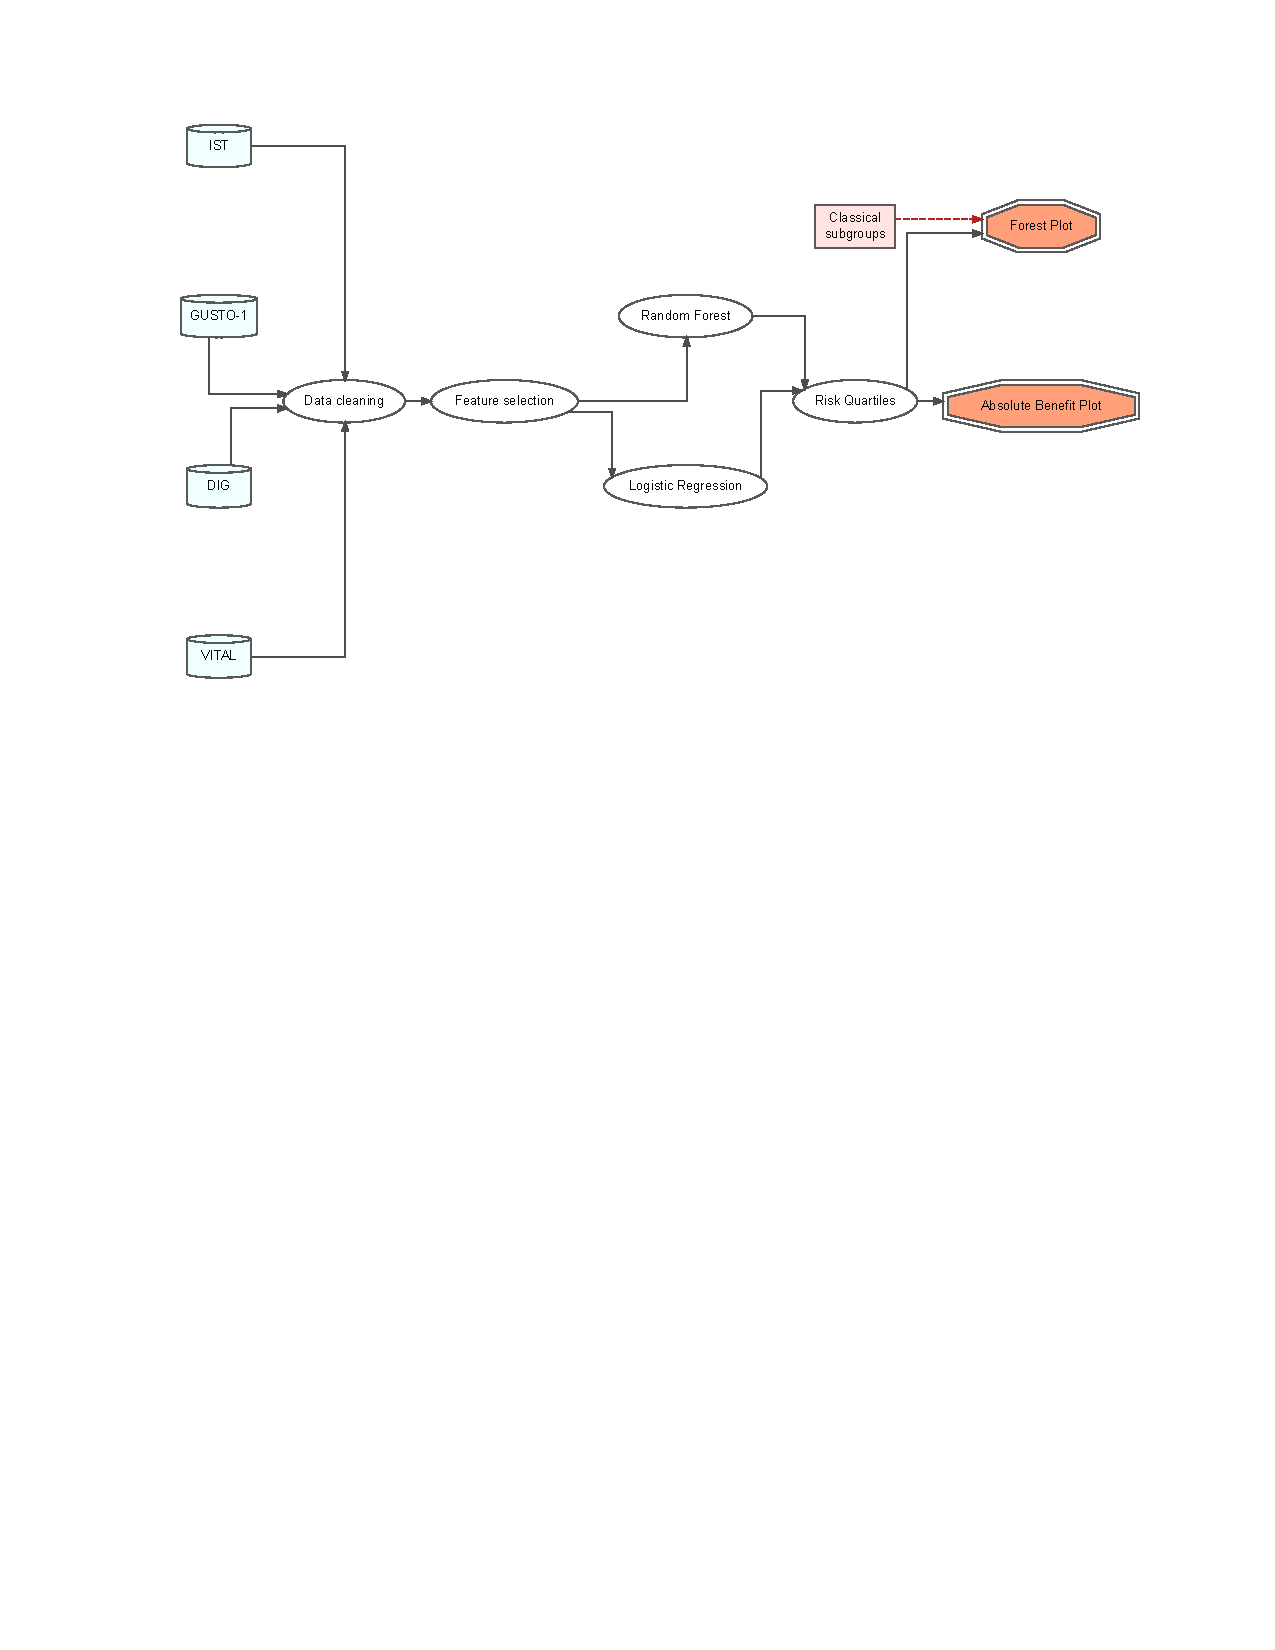
\includegraphics[keepaspectratio]{PATH---Thesis_files/figure-latex/unnamed-chunk-2-1.pdf}}

\section{Results}\label{results}

\subsection{Trial Characteristics}\label{trial-characteristics}

\subsection{Relative Treatment
Effects}\label{relative-treatment-effects}

\begin{verbatim}
## Loading required package: metadat
\end{verbatim}

\begin{verbatim}
## Loading 'meta' package (version 8.2-1).
## Type 'help(meta)' for a brief overview.
\end{verbatim}

\pandocbounded{
\includegraphics[keepaspectratio]{PATH---Thesis_files/figure-latex/unnamed-chunk-3-1.pdf}}

\subsection{Absolute Treatment
Effects}\label{absolute-treatment-effects}

\pandocbounded{
\includegraphics[keepaspectratio]{PATH---Thesis_files/figure-latex/unnamed-chunk-4-1.pdf}}

\section*{References}\label{references}
\addcontentsline{toc}{section}{References}

\phantomsection\label{refs}
\begin{CSLReferences}{1}{0}
\bibitem[\citeproctext]{ref-albertAssessingTreatmentEffect2005}
Albert, Jeffrey M., Gary L. Gadbury, and Edward J. Mascha. 2005.
{``Assessing Treatment Effect Heterogeneity in Clinical Trials with
Blocked Binary Outcomes.''} \emph{Biometrical Journal. Biometrische
Zeitschrift} 47 (5): 662--73.
\url{https://doi.org/10.1002/bimj.200510157}.

\bibitem[\citeproctext]{ref-kentPredictiveApproachesTreatment2020}
Kent, David M., David van Klaveren, Jessica K. Paulus, Ralph D'Agostino,
Steve Goodman, Rodney Hayward, John P. A. Ioannidis, et al. 2020. {``The
{Predictive Approaches} to {Treatment} Effect {Heterogeneity} ({PATH})
{Statement}: {Explanation} and {Elaboration}.''} \emph{Annals of
Internal Medicine} 172 (1): W1--25.
\url{https://doi.org/10.7326/M18-3668}.

\bibitem[\citeproctext]{ref-willkeConceptsTheoryEvidence2012}
Willke, Richard J., Zhiyuan Zheng, Prasun Subedi, Rikard Althin, and C.
Daniel Mullins. 2012. {``From Concepts, Theory, and Evidence of
Heterogeneity of Treatment Effects to Methodological Approaches: A
Primer.''} \emph{BMC Medical Research Methodology} 12 (December): 185.
\url{https://doi.org/10.1186/1471-2288-12-185}.

\end{CSLReferences}

\bibliographystyle{unsrt}
\bibliography{MSc -Thesis.bib}


\end{document}
